\chapter{Casos de Estudo}
Apresentar algumas topologias de estudo, mostrar resultados preliminares com o Rocs para o sistema de teste, mostrar algumas redes (pedir permiss�o para a AES?)

Nesta etapa foram realizados testes da metodologia proposta considerando
v�rios cen�rios operacionais de desarmes de alimentadores, incluindo defeitos a
montante ou a jusante dos equipamentos telecomandados para diferentes per�odos
de carga.
Para tanto, implementou-se a metodologia em um sistema prot�tipo,
desenvolvido em linguagem C++, a fim de avaliar o desempenho e a efic�cia do
sistema, bem como identificar as adequa��es necess�rias.
A Figura 2.10 ilustra a tela inicial do sistema, onde os n�s em cor azul
representam os equipamentos telecomandados NF (normalmente fechado) e os de
cor vermelha os equipamentos NA (normalmente abertos). Tamb�m h� a indica��o8
dos valores de corrente em cada trecho.

\begin{figure}[h]
\begin{centering}
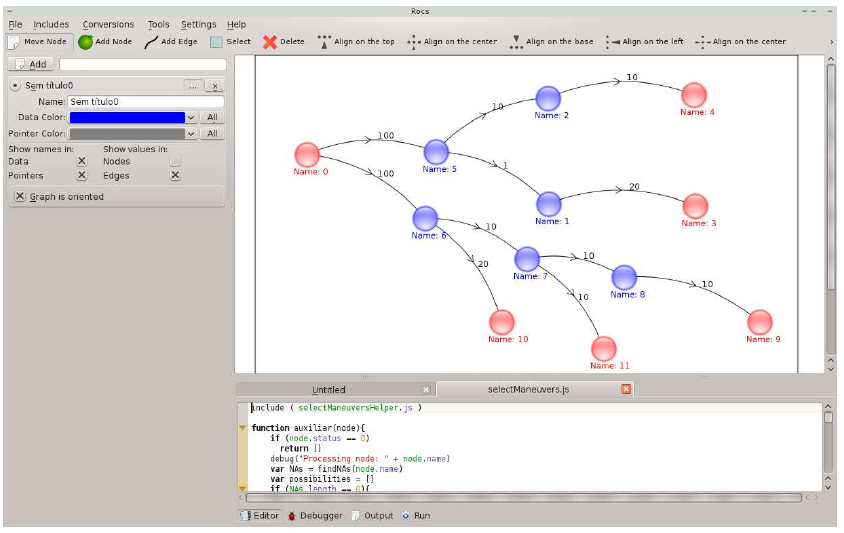
\includegraphics[width=0.6\columnwidth]{img/rocsTela1}
\par\end{centering}
\caption{Topologia inicial do caso de teste.\label{fig:Exemplorede}}
\end{figure}
Figura 2.10 - Tela inicial do sistema.

Para ilustrar a aplica��o do sistema ser�o apresentados dois estudos de
casos. No primeiro caso, considerou-se os defeitos nos trechos ``0 - 5'' e ``0 - 6'', e
analisou-se as transfer�ncias de carga realizadas pela metodologia proposta. Para o
defeito no trecho ``0 - 5'', o sistema abriu o equipamento do n� ``5'', isolando o
defeito, e fechou o equipamento do n� ``3'', restabelecendo a energia para as cargas
a jusante do defeito. J� para o defeito no trecho ``0 - 6'', o sistema abriu o
equipamento do n� ``6``, isolando o defeito, e fechou o equipamento do n� ``10'',
restabelecendo a energia para as cargas a jusante do defeito (Figura 2.11).

\begin{figure}[H]
\begin{centering}
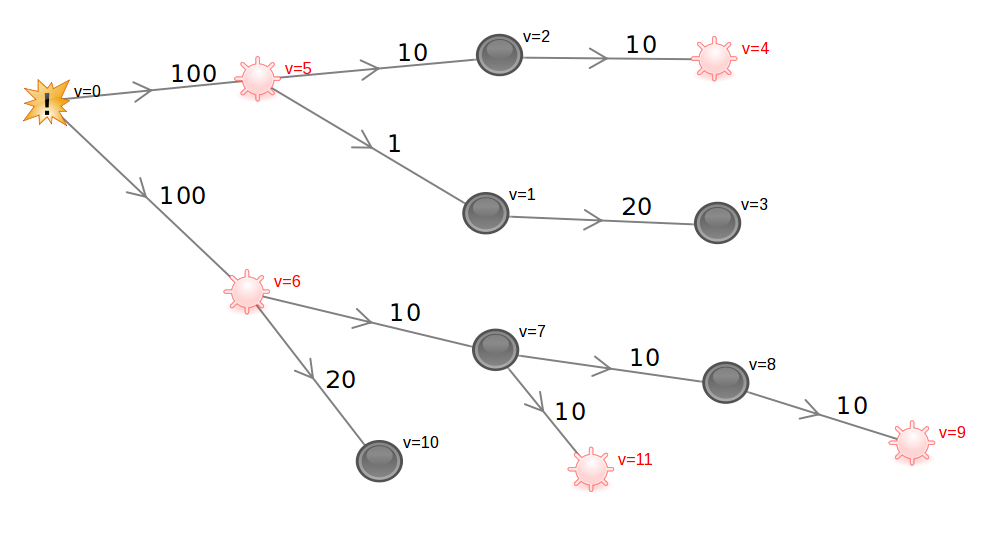
\includegraphics[width=0.6\columnwidth]{img/rocsTela2}
\par\end{centering}
\caption{Resultado do estudo do caso 1.\label{fig:Exemplorede}}
\end{figure}
No segundo caso, aumentou-se os valores de corrente nos trechos e colocou-
se como restri��o o limite de 99 A para os alimentadores assumirem carga. A
proposta � verificar se o sistema realizar� mais do que uma manobra para transferir
as cargas a jusante do defeito, isto �, se dividir� as mesmas entre os alimentadores
que podem assumir para evitar a viola��o da restri��o.
De acordo com a Figura 2.12 verifica-se que a metodologia respondeu de
forma satisfat�ria. Para o defeito no trecho ``0 - 5'', o sistema abriu os equipamentos
dos n�s ``5'' e ``1'', fechando os n�s ``4'' e ``3'', de modo a transferir parte da carga para
um alimentador e parte para o outro, evitando assim a viola��o da restri��o. J� para
o defeito no trecho ``0 - 6'', o sistema abriu os equipamentos dos n�s ``6'' e ``8'',
fechando os n�s ``10'' e ``9'', de modo a transferir parte da carga para um alimentador
e parte para o outro, evitando assim a viola��o da restri��o.
\begin{figure}[H]
\begin{centering}
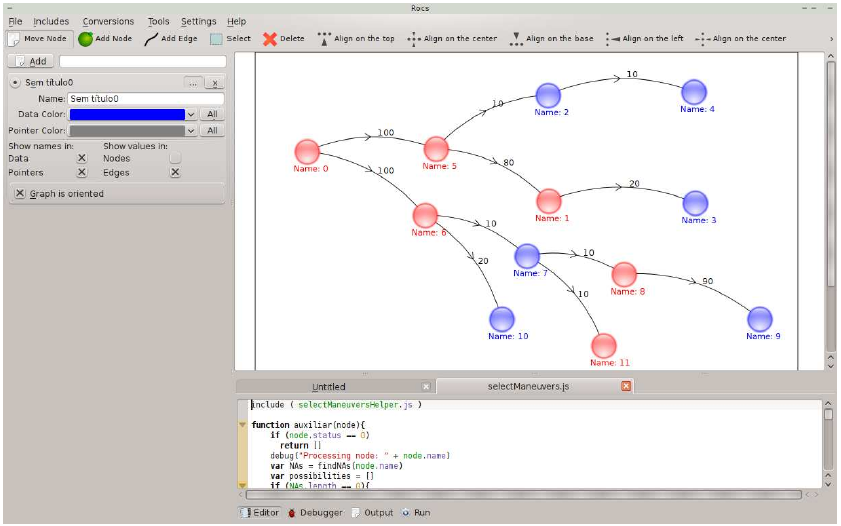
\includegraphics[width=0.6\columnwidth]{img/rocsTela3}
\par\end{centering}
\caption{Resultado do estudo do caso 2.\label{fig:Exemplorede}}
\end{figure}

\section{Resultados Obtidos}
Mostrar alguns resultados de redes reais. Necess�rio casos fict�cios?